\chapter{Introduction}

Prefetching instruction and data has taken a central position in processor architecture. This thesis squarely focuses on data prefetching. Data prefetching can be carried out in two possible ways, namely through hardware prediction of access stream and through the assistance of compiler-inserted prefetch instructions guided by static analysis or profile passes. While the former is known as hardware prefetching, the latter is known as software prefetching. This thesis deals with a certain class of hardware data prefetching. In this chapter, we first present an overview of a typical hardware data prefetcher. Next, we briefly introduce the concept of delinquent or critical loads leading to the problem statement of the thesis and our approach to the problem. We conclude this chapter with an outline of the thesis.

\section{ An Overview of a Typical Hardware Prefetcher }
Making predictions about future behaviour of a program is at the core of many of the microarchitecture techniques like cache replacement policies, branch predictors, etc..
Data prefetching is also one such prediction technique that fetches data required in advance by learning the past memory access behaviour of a program. Data prefetchers predict and fetch addresses of the access stream into the cache hierarchy. The position where a data prefetcher sits in the cache hierarchy can differ from one design to another. In this thesis, we will consider a simple design where a data prefetcher is attached to the last-level of the private cache hierarchy of each core.
\begin{figure}[H]
{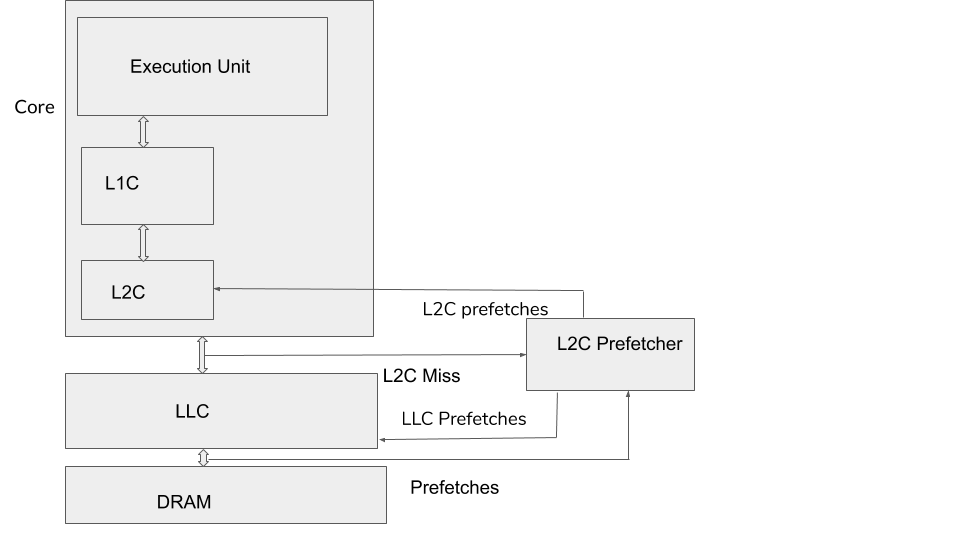
\includegraphics[scale=0.5]{images/L2CPrefetcher.png}}
\caption{Typical L2C prefetcher }\label{fig:L2CPrefetcher}
\end{figure}

There are many types of data prefetchers like next-line, stream buffers-based, history-based, etc.. Each one uses a different technique to predict the address stream of the program data. At a high level, two broad categories of data prefetchers exist. One category that attempts to discover patterns in the data address stream from the control flow of the program uses the instruction pointers~(IPs) of static load instructions for tagging prefetch patterns. These IP-based prefetchers discover the data address pattern for each static load instruction associated with an IP. One popular pattern that a prefetcher looks for is the delta between two consecutive load addresses sourced by the same static load instruction at an IP. This pattern is also known as the stride pattern. The other category of prefetchers exploits data flow of the program and uses the data addresses for tagging prefetch patterns. The stride or delta pattern is also popular among this class of prefetchers. There are also prefetchers that have used a combination of IPs and data addresses to discover and tag prefetch patterns.

A prefetch request can be triggered at numerous events. One commonly used trigger event is a cache miss. The prefetch requests for a sequence of addresses are sent out following the request for the address that has missed in the cache. Similarly, at other events, a prediction can be made and the predicted address sequence can be sent as prefetch requests.

Figure ~\ref{fig:L2CPrefetcher} describes the basic operations of a typical hardware prefetcher attached to the private L2 cache~(L2C). Generally, the L2C prefetcher prefetches all data blocks up to L2C only. Intelligent pefetchers can filter out less important  prefetches and put them only in the larger last-level cache~(LLC), while more critical blocks are sent further into the cache hierarchy up to the L2C.
Basic types of prefetchers just prefetch one or some of the next few blocks for a missed address with a fixed or a dynamic stride. The number of prefetch requests sent out together is usually referred to as the degree or depth of the prefetcher. Smart prefetchers adaptively modulate the depth. They can also select between a set of stride or delta values based on a dynamically learned confidence.

Various metrics and terminology used in prefetching literature are introduced below.

\begin{itemize}
\item Timeliness: A block should be ideally prefetched just in time synchronized with a demand access to the block from the CPU. An early prefetched block has a high chance of getting replaced from the cache before getting accessed. A late prefetched block fails to hide the latency of a miss completely. However, depending on how late a prefetch is a fraction of the miss latency can be saved.

\item Accuracy: The accuracy of a prefetcher is the ratio of the number of prefetched blocks that are used to the total number of prefetched blocks.

\item Coverage: Coverage of a prefetcher is the ratio of the total number of demand misses that are eliminated by the prefetcher to the total number of demand misses generated without using the prefetcher.

\item Lookahead or Degree or Depth: Lookahead or degree or depth is the number of prefetch requests generated together whenever the prefetcher is triggered.

\item Cache pollution: Unwanted or less important cache blocks that gets prefetched into the cache can replace useful blocks and pollute the cache degrading the performance.
\end {itemize}


\section{An Overview of Delinquent/Critical Loads}

Certain static loads or certain memory addresses may be more important for performance than others. These static load IPs or data addresses should 
be given more importance while prefetching.
Previous works have shown that there are only a small number of addresses that are responsible for most of the memory stalls arising from cache misses. It has been shown that out of all commit stalls, 60\% of the stalls are caused by a small set of loads~\cite{performance oriented prefetching}. These loads are called Loads Incurring Majority of Commit Stalls~(LIMCOS). Subsequent studies further classified these loads and termed the more important loads as delinquent loads~\cite{Long-range prefetching}. These loads are responsible for most of the cache misses. It was found that ten or fewer static loads cause more than 80\% of L1 data cache misses.
In this thesis, we use two measures of criticality of static loads: (i) the time for which the re-order buffer~(ROB) head remains blocked by a load instruction waiting to be retired and (ii) the number of instructions that are dependent on a load instruction.


\section{Brief Problem Statement}

Most of the prefetchers don’t use criticality information while learning prefetchable patterns or prefetching. However, prefetching only critical loads may result in similar or better performance with less consumption of bandwidth.
The main objective of the thesis is to use criticality information to extract important IPs corresponding to the set of performance-critical static loads and use them in tuning prefetcher parameters. We evaluate our proposal in terms of performance, bandwidth consumption, and other metrics. Achieving these objectives
involves various challenges discussed below. 
\begin{itemize}
\item Deciding criticality threshold values for ROB head block time and count of dependents on a load or designing any other mechanism to effectively compute them at run-time.

\item Using this criticality information in the underlying prefetcher and making changes to the prefetching algorithm to use this information effectively.

\item Reducing cache pollution while maintaining performance with less bandwidth.

 \end{itemize}
 
 \section{Outline of Our Approach}
 
We dynamically determine the set of critical static load IPs using the criticality metrics outlined above~(i.e., ROB head stall and dependence count) and use only those IPs for prefetch injection.
To obtain the optimal values of thresholds related to ROB head stall and dependencies, we use an empirical approach.

We use the signature path-based prefetcher~(SPP) as the underlying baseline prefetcher~(this prefetcher is discussed in detail in the next chapter). We predict lookahead depth for critical IPs using our own techniques instead of the in-built mechanism of SPP.
We predict the lookahead depth using parameters such as prefetch accuracy of a static load sourced by an IP and prefetch accuracy at the L2C and LLC with additional techniques that help effectively measure these parameters. We aim at maintaining or improving SPP performance while consuming less bandwidth and other resources.
To meet this goal, we have designed two separate techniques that change the underlying prefetcher in different ways. One design is less aggressive and consumes less bandwidth while maintaining the performance of SPP. The other design is more aggressive resulting in higher bandwidth consumption and better performance compared to the underlying prefetcher.
We have conducted extensive empirical evaluation to reach the optimal parameter setting and demonstrated the effects of prefetching based on critical IPs in various different scenarios.

\section{Organization of the Thesis}
\begin{itemize}
    \item \autoref{Chapter2} discusses the related work on critical loads and prefetching that we make use of in this thesis.
    \item \autoref{Chapter3:Recording ROB delay and ROB dependencies} discusses in detail the ROB head stall and dependence counts and the techniques we use to measure and record them at run-time.
    \item \autoref{Chapter4:Methods to predict Look ahead depth for critical delays}  discusses various techniques that we use to optimally decide the various threshold values and to efficiently measure and use various parameters like IP-based prefetch accuracy at L2C and LLC. It also discusses the different techniques that we design for low and high bandwidth settings.
    
    \item \autoref{Chapter5:Experiments and Results} demonstrates and discusses single-core and multi-core simulation results. 
    
    \item  \autoref{Chapter6:Conclusion and Future Work} concludes the thesis and points to some ideas for the future work.
\end{itemize}







